\section{Background and Motivating Example}
\label{sec:background}

% [M1]
In this section, we explain how dynamic typing and duck typing in Python
affect type-error detection. We then introduce Hoare triples and explain
how their preconditions and postconditions can summarize function behavior.

\subsection{Dynamic Typing and Duck Typing in Python}

% [M2]
A type-error detector must determine which types an operation's operands
can have and check whether the operation supports those
types~\cite{oh2024pyinder}. Python's dynamic typing and duck typing
complicate these tasks. With dynamic typing, the values used by an
operation may have different types on different executions.
Under duck typing, objects of different classes can support the same
operation. To check compatibility, a detector must examine whether the
operands meet the requirements of the methods or protocols used by that
operation. Moreover, the same operation may invoke different
implementations for different operand types. These implementations may
return values of different types, affecting the types used by subsequent
operations.

% [M3]
More specifically, \textbf{dynamic typing} allows both local and global
variables in Python to be bound to objects of different
types during program execution~\cite{pythonExecutionModel,pythonDataModel}.
Consequently, an operand's type depends on the assignments and updates
along the execution path to the operation.
% [M4]
Function calls can also change the values that a caller uses. A caller may
assign a function's return value to a variable. A callee may also update a
global variable or an attribute of an object shared with its caller.
When the caller next reads the updated variable or attribute, it may
obtain a value of a different type, even if the callee did not return that
value. To determine the types used by subsequent operations, a detector
must therefore track assignments and updates both within functions and
across calls.

% [M5]
In Python, code written in the \textbf{duck typing} style uses objects
through the methods and attributes they support, without requiring them
to belong to a particular class~\cite{pythonGlossary}.
For an operation that calls a method on an operand, a detector must check
that the object supports that method and that the call satisfies the
method's requirements.
% [M6]
Beyond checking whether an operation accepts its operands, a detector
must account for what its implementation returns or updates. Python's
dispatch rules may select different implementations for different operand
types. These implementations may return values of different types or
update state that subsequent operations read. The detector must track
these effects because later operations use the resulting values and
updated state.

% [M7]
To check subsequent operations precisely, a detector can relate the types
and state before each operation to its result and the state after it.
For a function call, this relation connects the argument types and the
types of shared values before the call to the return type and the types
of updated values after it. The shared values include global variables
and object attributes that the function reads or updates.
The same function may return or update values of different types under
different calling conditions or along different execution paths. If the
detector records only the possible resulting types, it loses the
conditions under which each type arises. It may then consider types that
cannot occur in the current calling context when checking a later
operation. Keeping each result associated with its conditions allows the
detector to use the type information relevant to that call.

\subsection{Hoare Triples as Function Summaries}
\label{sec:hoare-background}

% [M8]
To check operations after a call, a detector must account for the values
returned or updated by the callee. A function summary describes the
callee's relevant behavior so that the detector can reuse it at call
sites. For type-error detection, a summary can relate conditions on the
arguments and shared state before the call to type facts that hold after
it returns normally. Hoare triples provide a standard way to express
this relationship between conditions before and after execution.

Hoare logic describes how executing a program changes its
state~\cite{hoare1969axiomatic,softwareFoundationsHoare}. A Hoare triple has
the form
\begin{equation}
\{P\}\ C\ \{Q\},
\label{eq:hoare-triple}
\end{equation}
% [M9]
where $C$ is a command, and $P$ and $Q$ are assertions over program states,
called the precondition and postcondition, respectively. An assertion
describes a property of a state, such as the type of a value held in a
variable.
% [M10]
We use a partial-correctness interpretation that describes what holds on
normal termination. A valid triple states that if $P$ holds before $C$
executes and $C$ terminates normally, then $Q$ holds afterward. In other
words, $P$ gives the assumptions under which executing $C$ establishes $Q$
on normal termination. Under this interpretation, the triple does not
guarantee that $C$ terminates or executes without raising a
\texttt{TypeError}.

% [M11]
When a Hoare triple is used as a function summary, its precondition can
express assumptions about the arguments and shared state, while its
postcondition can describe the return value and properties of the shared
state after the call.
% [M12]
To apply the summary at a call site, the detector matches the callee's
parameters with the caller's arguments and interprets references to
shared objects in the caller's state. This step instantiates the summary
for the call. If the calling state satisfies the instantiated
precondition, the postcondition gives facts that hold when the call
returns normally. The detector can use these facts to check subsequent
operations. If the calling state does not satisfy the precondition, the
detector cannot rely on this guarantee. That alone does not establish a
type error. To determine whether an error occurs, the detector must
examine the relevant operations and their exceptional behavior.

% [M13]
Hoare triples also support sequential composition. If
$\{P\}\ C_1\ \{R\}$ and $\{R\}\ C_2\ \{Q\}$ are valid, then
$\{P\}\ C_1; C_2\ \{Q\}$ is valid. Here, $R$ is an intermediate assertion.
Starting from a state satisfying $P$, $C_1$ establishes $R$ on normal
termination. This assertion then serves as the precondition for the
second triple. Thus, the properties established by
one command provide the assumptions for reasoning about the next command.

% [M14]
For Python type-error detection, a detector can use a function summary to
update the type facts it uses after a call. If a function updates an
attribute of a shared object, its postcondition can describe the type of
the value held in that attribute on normal return. The caller still
accesses the same object, but the attribute now holds the updated value.
A type fact about its previous contents may therefore no longer apply.
The detector must check subsequent operations using type facts that
account for the update. When the calling state satisfies the summary's
precondition, its postcondition can provide these facts.

% [R01]
\subsection{Motivating Example}
\label{sec:motivating-example}

% [R02]
Figure~\ref{fig:motivating-example} presents a message-processing
example that illustrates the need to track type-state changes across
function calls. The function \texttt{make\_line} calls
\texttt{encode\_message} to encode a message body before appending
a newline. The body is declared as \texttt{str | bytes}.
For a string body, \texttt{encode\_message} invokes the supplied
encoder and stores its result in the same message object.
\texttt{TextEncoder} returns the string unchanged, whereas
\texttt{Utf8Encoder} converts it to bytes.

% [R02a]
As shown in the figure, Mypy, Pyrefly, and Pyright do not report the
concatenation error, whereas PyTT detects it. Analyzing this example
reveals two related requirements for type-error detection. First,
the analyzer must propagate changes to the shared message body across
the call so that the subsequent operation is checked against its
updated type. Second, distinguishing the failing UTF-8 call from the
safe text-encoder call requires retaining the conditions under which
each update occurs. We examine these requirements below and explain
how PyTT addresses them through conditional type-state summaries.

\begin{figure}[!htbp]
\centering
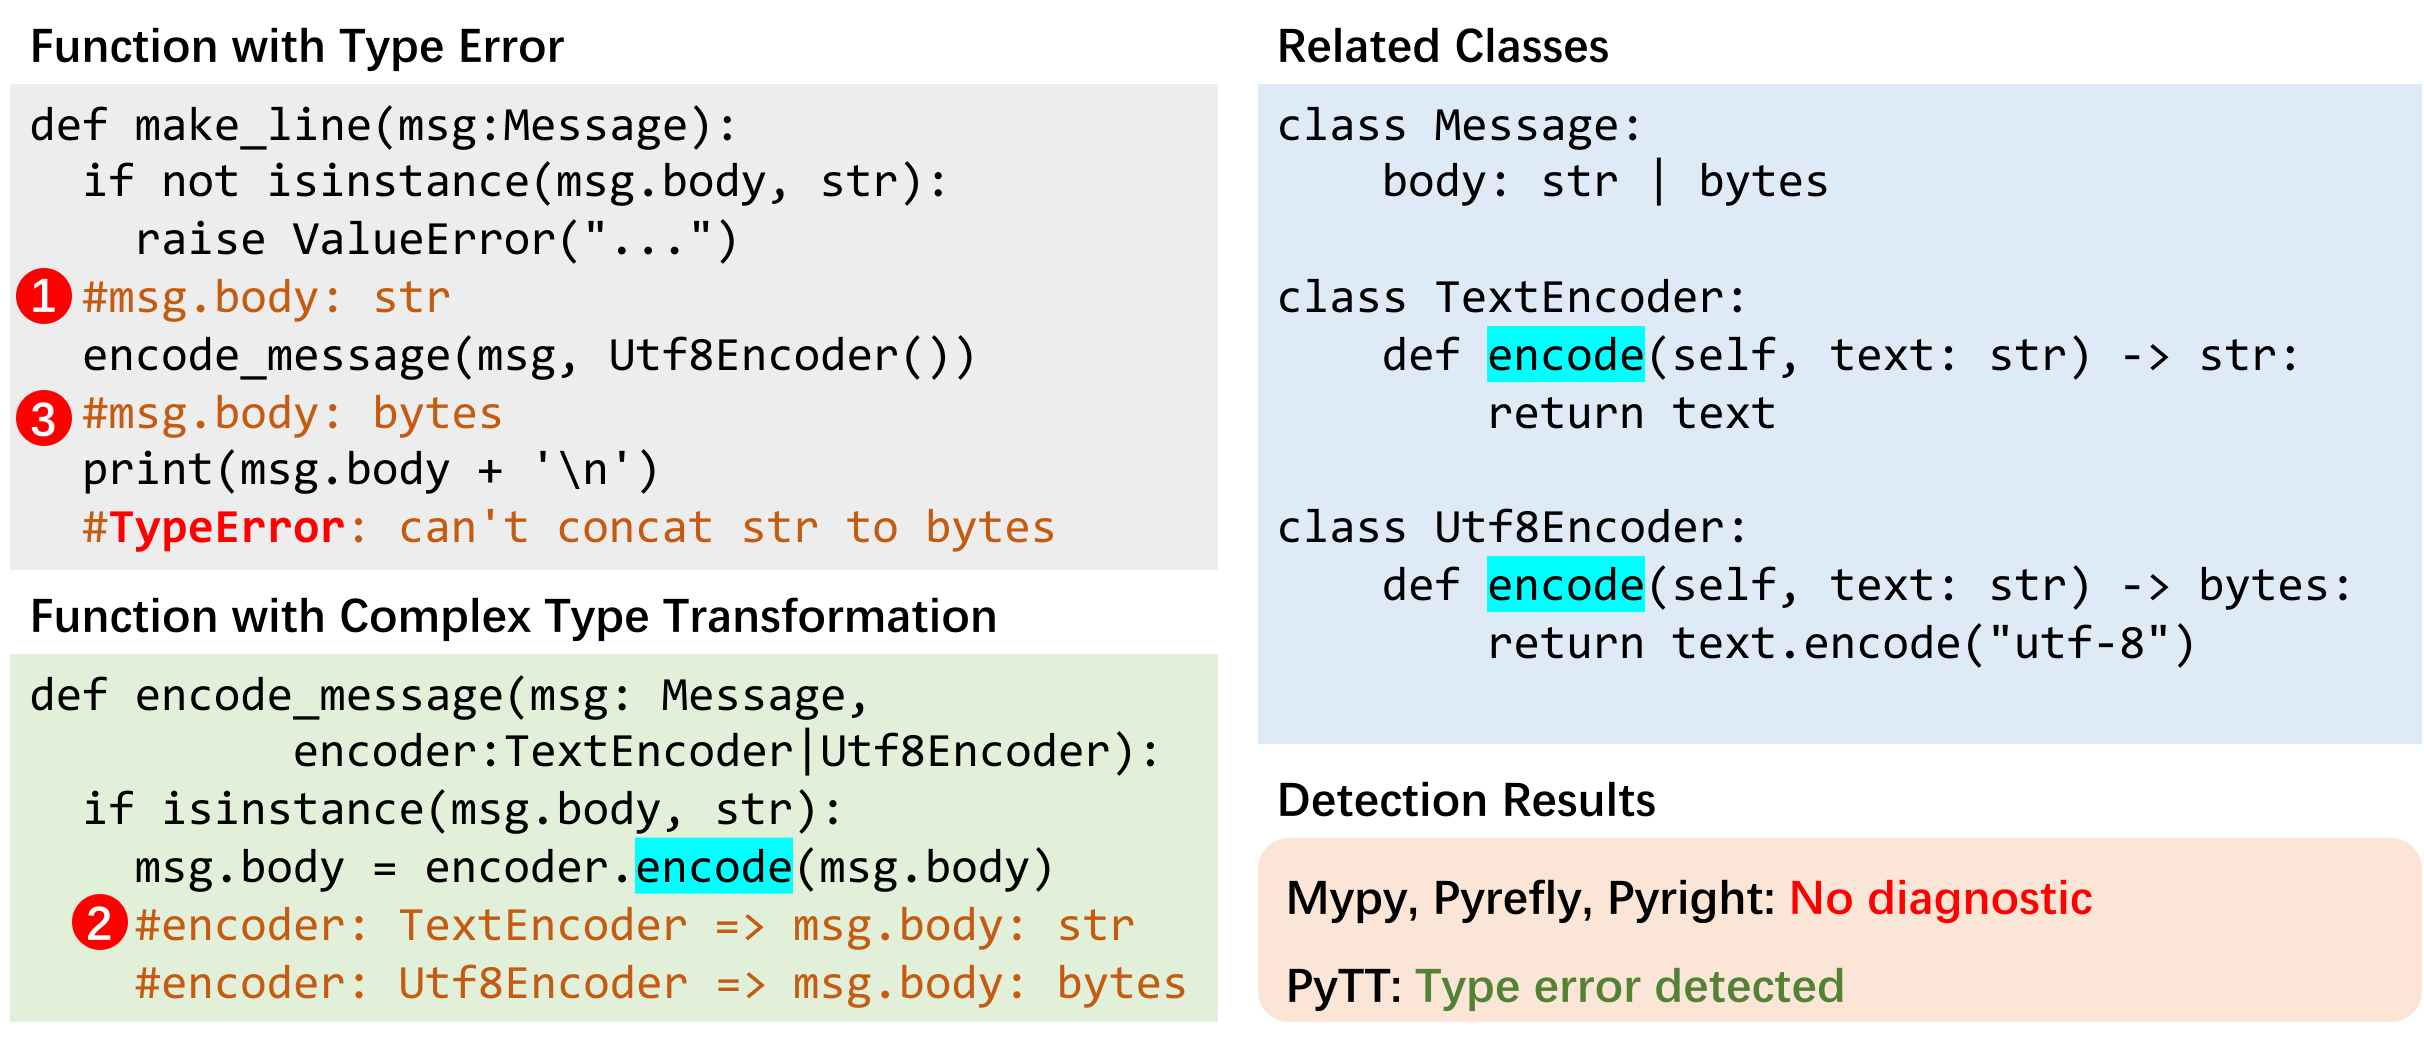
\includegraphics[width=\linewidth]{photos/motivatingExample.png}
% [R03]
\caption{Motivating example of interprocedural type-state changes
and type-error detection results.}
\Description{The caller make_line rejects a non-string message body,
then calls encode_message with Utf8Encoder and attempts to concatenate
msg.body with a newline string. For a string input, the helper writes
the encoder's result into the same message object. TextEncoder returns
a string, and Utf8Encoder returns bytes. Points 1, 2, and 3 mark the
string body before the call, the conditional field updates, and the
bytes body after the UTF-8 call returns normally. The concatenation
then raises TypeError. The result panel labels Mypy, Pyrefly, and
Pyright with No diagnostic and PyTT with Type error detected.}
\label{fig:motivating-example}
\end{figure}

% [R04]
\textbf{(1) Interprocedural Type-State Propagation.}
In \texttt{make\_line}, the guard raises \texttt{ValueError} when
\texttt{msg.body} is not a string. Thus, the body has type
\texttt{str} at point~1. The subsequent call passes \texttt{msg}
and a \texttt{Utf8Encoder} instance to \texttt{encode\_message},
which writes the encoding result into \texttt{msg.body}. Because
both functions access the same message object, the body has type
\texttt{bytes} at point~3 after the call returns normally.
The expression \texttt{msg.body + '\textbackslash n'} then raises
\texttt{TypeError} before \texttt{print} is invoked, and the exception
escapes \texttt{make\_line}.

% [R05]
Both the original string and the updated bytes satisfy the field's
union annotation, but the updated body does not support concatenation
with a string. Detecting this error requires propagating the field
update from \texttt{encode\_message} to its caller. The function's
return type, \texttt{None}, does not describe this update. If the
analyzer retains the string type established at point~1, it can miss
the error at point~3.

% [R06]
\textbf{(2) Conditional Type-State Modeling.}
Propagating a field update also requires determining which type the
call establishes. In this example, that type depends on the encoder
argument. Replacing \texttt{Utf8Encoder} with
\texttt{TextEncoder} leaves a string body and makes the concatenation
valid. An analyzer that assigns \texttt{str | bytes} to the body
after either call can flag the potential bytes/string conflict.
However, retaining the bytes alternative for \texttt{TextEncoder}
can also cause a false alarm. Distinguishing these calls therefore
requires preserving the relation between the encoder argument and the
resulting field type under the incoming string condition.

% [R07]
PyTT addresses these requirements using path-sensitive type contracts
(PSTCs), which record field updates together with their calling
conditions and propagate the applicable updates to callers. At point~2,
the contract for \texttt{encode\_message} records two cases for an
incoming string body. On normal return, the \texttt{TextEncoder}
case establishes a string body, and the \texttt{Utf8Encoder} case
establishes a bytes body. For a non-string input, the function leaves
the body unchanged.

% [R08]
At the illustrated call, PyTT uses the string type established by the
guard and the \texttt{Utf8Encoder} argument to select the second case.
It maps the callee's message parameter to the caller's object and
updates the type of \texttt{msg.body} accordingly. The subsequent
concatenation is therefore checked with a bytes body, revealing the
type error.

